
The experiment was designed to get a better understanding about the contribution linear and angular velocity, oscillation angle, direction, and orientation to express happiness, anger, sadness and fear, which are four out of six emotions considered by Ekman~\cite{Ekman2004} as basic emotions.
%%%%%%%%%%%%%%%%%%%
%%%%%%%%%%%%%%%%%%%

\subsection{Independent Variables}

The definitions of the selected independent variables are reported here below.

\begin{itemize}
	\item \textbf{Angular velocity} is the rotational speed  ($\omega$) of the robot with respect to its center.

	\item \textbf{Oscillation angle} is the maximum extension in which the robot will rotate around its center in the oscillating movement ($\theta$).

	\item \textbf{Linear velocity} is the rate of change of the position of the robot ($V$). 

	\item \textbf{Direction with respect to participant's perspective} is the angle generated from the participant's point of view with respect to the robots trajectory ($D$).

	\item \textbf{Orientation of the body with respect to participant's perspective} is the robot's body orientation with respect to the robot's trajectory ($\phi$).

\end{itemize}

The three first variables are shown in Figure~\ref{fig:angular_movement}. As it could be observed, robot's frame of reference is draw to show that it could move straight while is rotating.


\begin{figure}
	\centering
	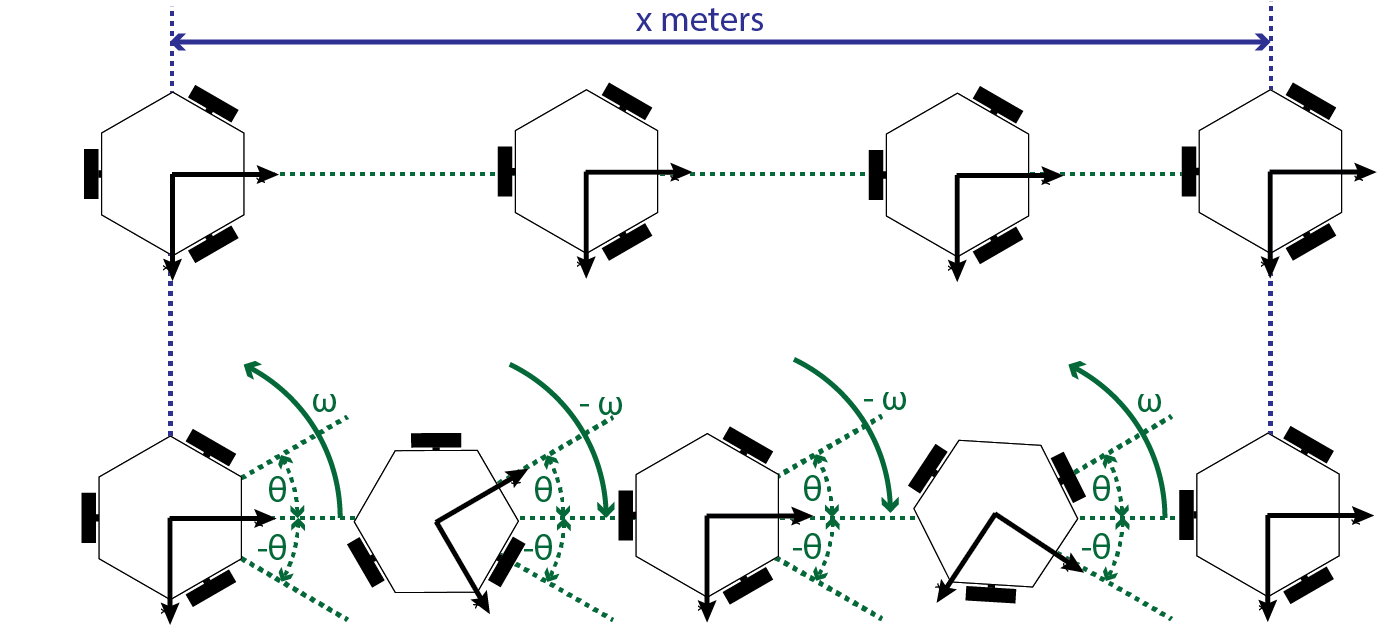
\includegraphics[width=0.48\textwidth]{./Images/ExampleMovement.png} 
	\caption{Example of the features used in the experiment. $x$ represents the displacement in meters, $\omega$ is the angular velocity ($rad/s$) and $\theta$ the oscillation of the body around its center ($rad$). The upper sequence depicts a movement based only on linear velocity, while the bottom one shows a sequence with angular and linear movement. The two black arrows in the robot's middle depict robot's frame of reference.}
	\label{fig:angular_movement}
	
\end{figure} 

%%%%%%%%%%%%%%%%%%%
%%%%%%%%%%%%%%%%%%%
\subsection{Dependent Variables}

\begin{itemize}
	\item \textbf{Emotion:} is the feeling perceived by the participants from the robot's movement. From previous experiences %TODO cite
	, it was decided to ask the participants to select an emotion name in a list including the four emotions intended to be expressed,  two mental states that could be misinterpreted from these emotions, and the option of ``other'', where participants could write their own interpretation. 
	The two  states of mind included as confounding terms are tenderness and excitement, which correspond to low and high arousal states.
	
	\item \textbf{Emotion's intensity:} indicate the emotion intensity as perceived by the subject. This variable is measured on a ten point scale rate, ranging from 0 to 10, where 0 means that the corresponding emotion is not perceived by the subject and 10 that the emotion is highly perceived by the subject. 

\end{itemize}
%%%%%%%%%%%%%%%%%%%
%%%%%%%%%%%%%%%%%%%
\subsection{Independents' Variables Values}

It was decided to select specific for all independents variables, discrete values to make the experiment feasible. First, a simple test to evaluate when significant changes could be perceived was performed on a small sample of independent subjects. Base on this test specific values for oscillation angle, and angular and linear velocities were selected. For the remaining two variables were selected the cases that could be beneficial for the experiment. 
The chosen values are shown in Table~\ref{table:variables_values}. 

\begin{table}[htb]
\centering
\caption{Possible values for each of the independent variables.}
\begin{tabular}{|c|c|c|c|c|}
\hline
\backslashbox{Variable}{Possibilities} & First & Second & Third & Fourth\\
\hline   
Angular Velocity ($rad/sec$)& $0$ & $1$ & $2$ & $3$\\
\hline
Oscillation Angle ($rad$)& $0$ & $0.087$ & $0.175$ & $0.349$\\
\hline
Linear Velocity ($mm/sec$) & $0$ & $200$ & $500$ & $900$\\
\hline
Direction ($rad$)&$0$&$\pi$&$\frac{-\pi}{2}$& \\
\hline
Orientation ($rad$) & $0$ & $\pi$ & & \\
\hline 
\multicolumn{5}{c}{}
\end{tabular} 
\label{table:variables_values}
\end{table}

To get a better idea about the Direction and Orientation values, in Figure~\ref{fig:possibilities_orientation_direction} are reported all the possibilities for these two variables.

\begin{figure}
	\centering
	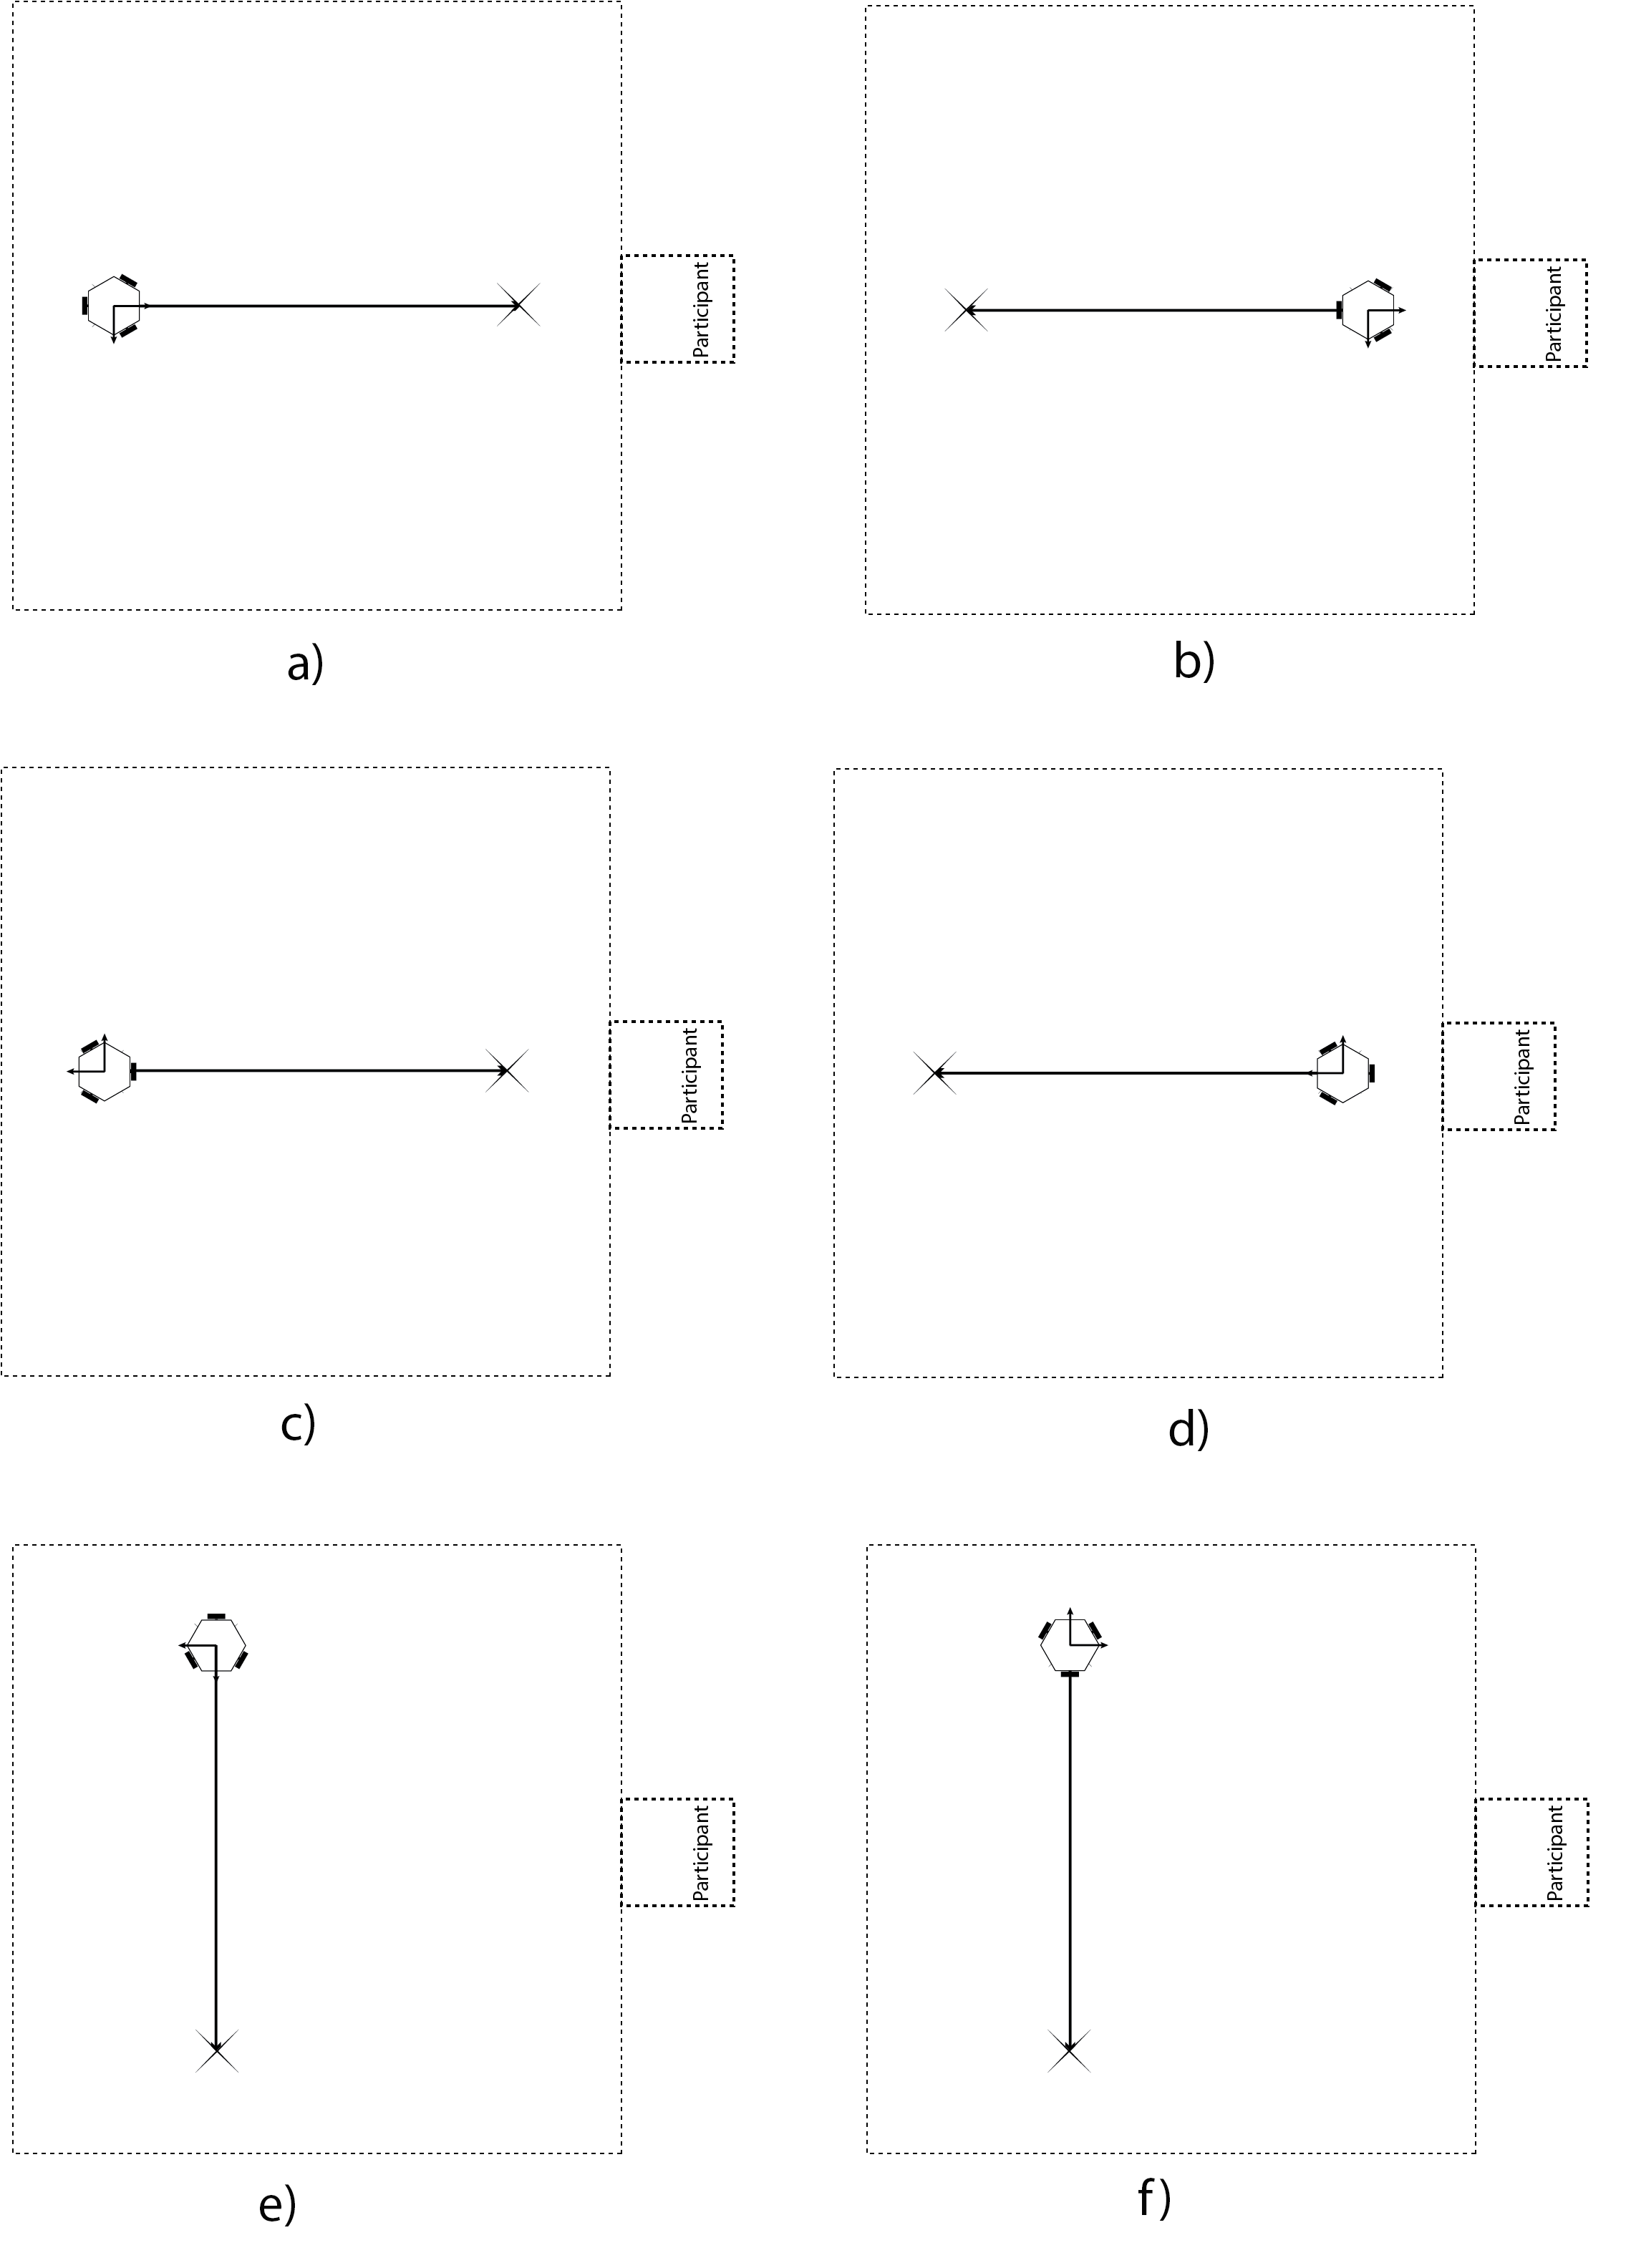
\includegraphics[width=0.48\textwidth]{./Images/possibilities_case.png} 
	\caption{Combination of direction and orientation. The crosses symbolize the final position. The robot represents the initial position with its orientation, which is represented through the robot's frame of reference. The dash big square represents robot's movement zone, while the small represents participant's zone. a) Direction = $0$ and Orientation = $0$. b) Direction = $0$ and Orientation = $\pi$. c) Direction = $\pi$ and Orientation = $\pi$. d) Direction = $\pi$ and Orientation = $0$. e) Direction = $\frac{-\pi}{2}$ and Orientation = $0$. f) Direction = $\frac{-\pi}{2}$ and Orientation = $\pi$}
	\label{fig:possibilities_orientation_direction}
\end{figure}

The experiences, meant as desired procedures to compare~\cite{oehlert2000first}, were generated from the combination of independent variables' values for a total of 384 combinations. All the experiences that would not add any significant information to the experiment were deleted, such as experiences with $\theta=0$ and $\omega \neq 0$, which reduced the total amount of treatments to 195.

%%%%%%%%%%%%%%%%%%%
%%%%%%%%%%%%%%%%%%%
\subsection{Participants' Sequence}

It was decided that each subject will be just exposed to twenty over one hundred and ninety five possible experiences, which lasted  from 10 to 15 minutes. This was decided because each subject was a volunteer and would not perceive any monetary remuneration, so the time dedicated to the experiment had to be kept limited. The twenty treatments were selected picking a number without replacement from 1 to 195.
%%%%%%%%%%%%%%%%%%%
%%%%%%%%%%%%%%%%%%%

\subsection{Setup}

The experiment's setup and dimensions are shown in the Figure~\ref{fig:setup}. The crosses symbolize possible starting points, which were selected depending on the direction's value, as it is showed in Figure~\ref{fig:possibilities_orientation_direction}. 

\begin{figure}
	\centering
	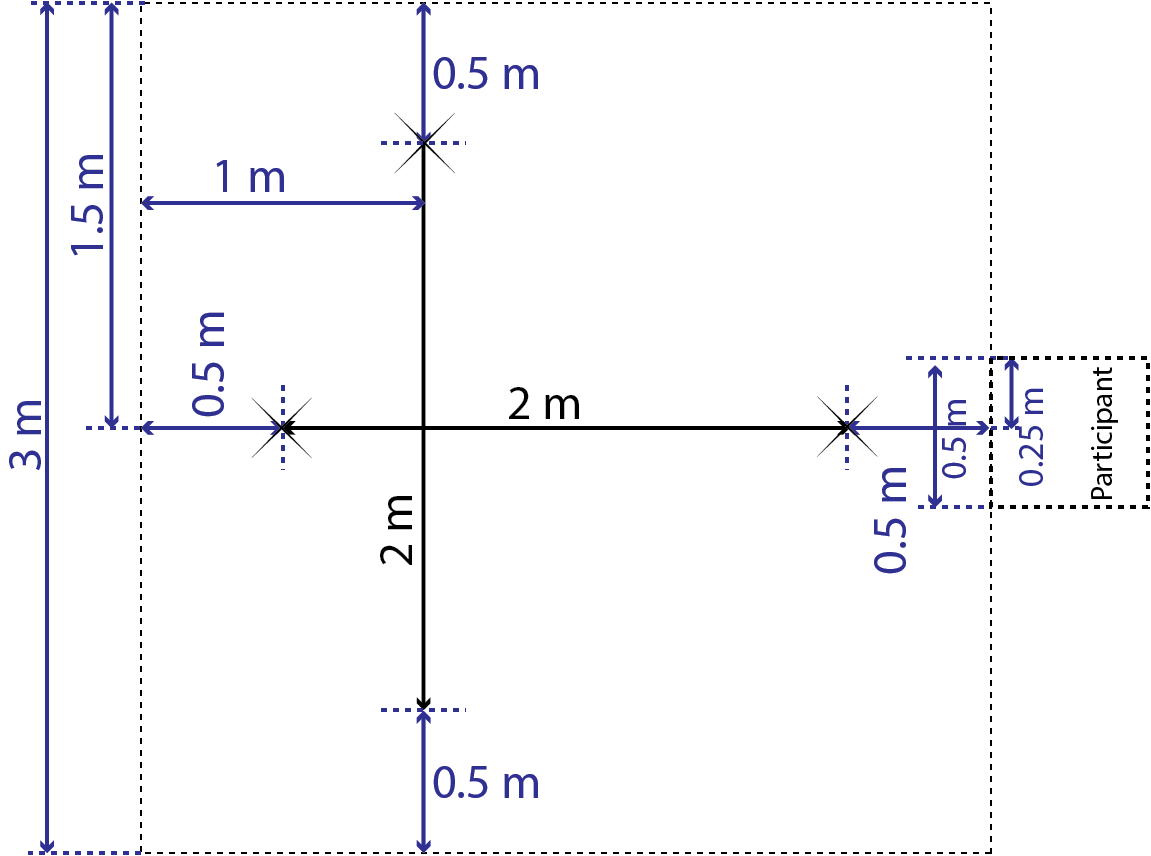
\includegraphics[width=0.45\textwidth]{./Images/ExperimentGeneral.png} 
	\caption{Setup for the experiment. The crosses symbolize the possible starting points.}
	\label{fig:setup}
\end{figure} 